% Icons : https://ctan.tetaneutral.net/fonts/fontawesome5/doc/fontawesome5.pdf
% Use the "normalphoto" option for a normal photo instead of cropped to a circle
%\documentclass[10pt,a4paper,ragged2e,withhyper]{altacv}
\documentclass[10pt,a4paper,ragged2e,withhyper,normalphoto]{altacv}

% Layout
\geometry{left=1.25cm,right=1.25cm,top=1.5cm,bottom=1.5cm,columnsep=1.2cm}

% The paracol package lets you typeset columns of text in parallel
\usepackage{paracol}

% Fonts
\iftutex
  % If using xelatex or lualatex:
  \setmainfont{Roboto Slab}
  \setsansfont{Lato}
  \renewcommand{\familydefault}{\sfdefault}
\else
  % If using pdflatex:
  \usepackage[rm]{roboto}
  \usepackage[defaultsans]{lato}
  % \usepackage{sourcesanspro}
  \renewcommand{\familydefault}{\sfdefault}
\fi

% Colours
\definecolor{SlateGrey}{HTML}{2E2E2E}
\definecolor{LightGrey}{HTML}{666666}
\definecolor{Carmine}{HTML}{960018}
\definecolor{EngineeringOrange}{HTML}{C80815}
\definecolor{GoldenMetallic}{HTML}{D4AF37}
\definecolor{Flax}{HTML}{EEDC82}
\definecolor{OldLace}{HTML}{FDF5E6}
\definecolor{DodgerBlue}{HTML}{1E90FF}
\definecolor{EgyptianBlue}{HTML}{0033AA}
\definecolor{ForestGreen}{HTML}{228B22}

\colorlet{name}{EgyptianBlue}
\colorlet{tagline}{DodgerBlue}
\colorlet{heading}{DodgerBlue}
\colorlet{headingrule}{SlateGrey}
\colorlet{subheading}{SlateGrey}
\colorlet{accent}{SlateGrey}
\colorlet{emphasis}{SlateGrey}
\colorlet{body}{LightGrey}

% Change the bullets for itemize and rating marker
% for \cvskill
\renewcommand{\cvItemMarker}{{\small\textbullet}}
\renewcommand{\cvRatingMarker}{\faCircle}
% for the date/location for \cvevent
\renewcommand{\cvDateMarker}{\faCalendar*[regular]}
\renewcommand{\cvLocationMarker}{\faMapMarker*}

% Infos
\begin{document}

\name{Heuze Florent}
\tagline{Chef de projet en Intelligence Artificielle}
\photoL{6cm}{heuzef_2025_01}
%\photoL{4cm}{heuzef_2025_portrait_min}

\personalinfo{
  \printinfo{\faCalendar}{1990}
  \location{Bordeaux, France}
  \email{contact@heuzef.com}
  \phone{+33(0)6 31 32 66 54}
  \homepage{heuzef.com}
  \linkedin{heuzef}
  %\github{heuzef}
}

\makecvheader

\cvsection{À propos}

\begin{quote}
``
Fort d'une expérience de 15 ans en tant que technicien IT, je me réoriente dans le domaine de la Data.

Animé par le partage et le travail d’équipe, je m’attache à l'analyse des besoins pour proposer des solutions alliant pertinence et excellence opérationnelle.

\medskip

Au fil de ma carrière, j’ai souvent joué un rôle de guide, aidant à structurer et à organiser les projets. 

Ma capacité à jouer un rôle de facilitateur entre différents experts me permet de créer un langage commun et d'optimiser la collaboration, contribuant ainsi à l'atteinte d'objectifs ambitieux et innovants.
''
\end{quote}

\bigskip

\columnratio{0.55}

\begin{paracol}{2}

\cvsection{Homologations}

\cvachievement{\faGraduationCap}{Machine Learning Engineer}{Datascientest, RNCP 36129 Niveau 7, 2025}

\cvachievement{\faGraduationCap}{Gestionnaire en Maintenance et Support Informatique}{CESI, RNCP 34602 Niveau 5, 2015}

\cvachievement{\faGraduationCap}{Technicien Supérieur Gestionnaire exploitant de Ressources Informatiques}{Site-Informatique, RNCP5918 Niveau 5, 2013}

\cvachievement{\faGraduationCap}{Conseiller et Assistant en Technologies de l'Information de de la Communication}{AFPA, RNCP4537 Niveau 4, 2011}

\divider

\cvachievement{\faCertificate}{AWS Certified Cloud Practitioner}{AWS, 2025}

\cvachievement{\faCertificate}{OpenCV Bootcamp}{OpenCV University, 2024}

\cvachievement{\faCertificate}{Chinois A1}{CCI Cognac (Lilate), 2023}

\cvachievement{\faCertificate}{CCNA1}{CISCO, 2013}

\cvachievement{\faCertificate}{Designer Graphiste}{Lignes et Formations, 2011}

\cvachievement{\faCertificate}{PSC1}{Croix-Rouge, 2005/2008/2012/2022}

\cvsection{Langues}

\cvachievement{\faFlag}{Français}{Natif}

\divider

\cvachievement{\faFlag}{Anglais}{B2}

\divider

\cvachievement{\faFlag}{Chinois}{A1}

\switchcolumn

\cvsection{Compétences}

\cvtag{Excellence opérationnelle {\color{GoldenMetallic}\faCogs}}\\
\cvtag{Autonome {\color{EngineeringOrange}\faDove}}
\cvtag{Motivateur {\color{Carmine}\faBullhorn}}\\
\cvtag{Écoute active {\color{EgyptianBlue}\faAssistiveListeningSystems}}
\cvtag{Résilient {\color{ForestGreen}\faTree}}
\\
\divider

\cvtag{AI {\color{black}\faBrain}}
\cvtag{Machine Learning {\color{GoldenMetallic}\faUserCog}}
\cvtag{Deep Learning {\color{GoldenMetallic}\faUserCog}}\\
\cvtag{Python {\color{ForestGreen}\faPython}}
\cvtag{MLFlow {\color{cyan}\faSync*}}
\cvtag{BentoML {\color{SlateGrey}\faLayerGroup}}
\\
\divider

\cvtag{Data {\color{black}\faDatabase}}
\cvtag{(No)SQL {\color{SlateGrey}\faCode}}
\cvtag{ETL {\color{SlateGrey}\faFileDownload}}
\cvtag{API {\color{EgyptianBlue}\faPlug}}
\cvtag{Scraping {\color{EgyptianBlue}\faSearch}}
\cvtag{Data Viz {\color{Carmine}\faChartPie}}
\cvtag{RGPD {\color{EgyptianBlue}\faGlobeEurope}}
\cvtag{AI Act {\color{GoldenMetallic}\faBalanceScale}}
\\
\divider

\cvtag{DevSecOps {\color{black}\faLinux}}
\cvtag{Git/DVC {\color{EngineeringOrange}\faCodeBranch}}\\
\cvtag{Conteneurisation {\color{EgyptianBlue}\faDocker}}
\cvtag{Orchestration {\color{Carmine}\faBoxes}}\\
\cvtag{Jenkins {\color{EngineeringOrange}\faJenkins}}
\cvtag{Airflow {\color{DodgerBlue}\faFan}}
\\
\divider

\cvtag{Réseaux TCP/IP {\color{black}\faNetworkWired}}
\cvtag{Hypervision {\color{EngineeringOrange}\faServer}}\\
\cvtag{IaC {\color{black}\faCode}}
\cvtag{Sécurité {\color{EgyptianBlue}\faShield*}}
\cvtag{Supervision {\color{Carmine}\faEye}}
\\
\divider

\cvtag{Infographie {\color{black}\faPalette}}
\cvtag{PAO {\color{Flax}\faPrint}}
\cvtag{CAO {\color{EngineeringOrange}\faCube}}
\cvtag{DAO {\color{SlateGrey}\faPencilRuler}}
\\
\divider

\cvtag{Web {\color{black}\faGlobe}}
\cvtag{Dev {\color{EngineeringOrange}\faHtml5}}
\cvtag{CMS {\color{DodgerBlue}\faWordpress}}
\cvtag{SSG {\color{Flax}\faSitemap}}
\\
\divider

\cvtag{Cloud {\color{black}\faCloud}}
\cvtag{AWS {\color{EngineeringOrange}\faAws}}
\\
\divider

\end{paracol}

\newpage

\begin{figure}
    \centering
    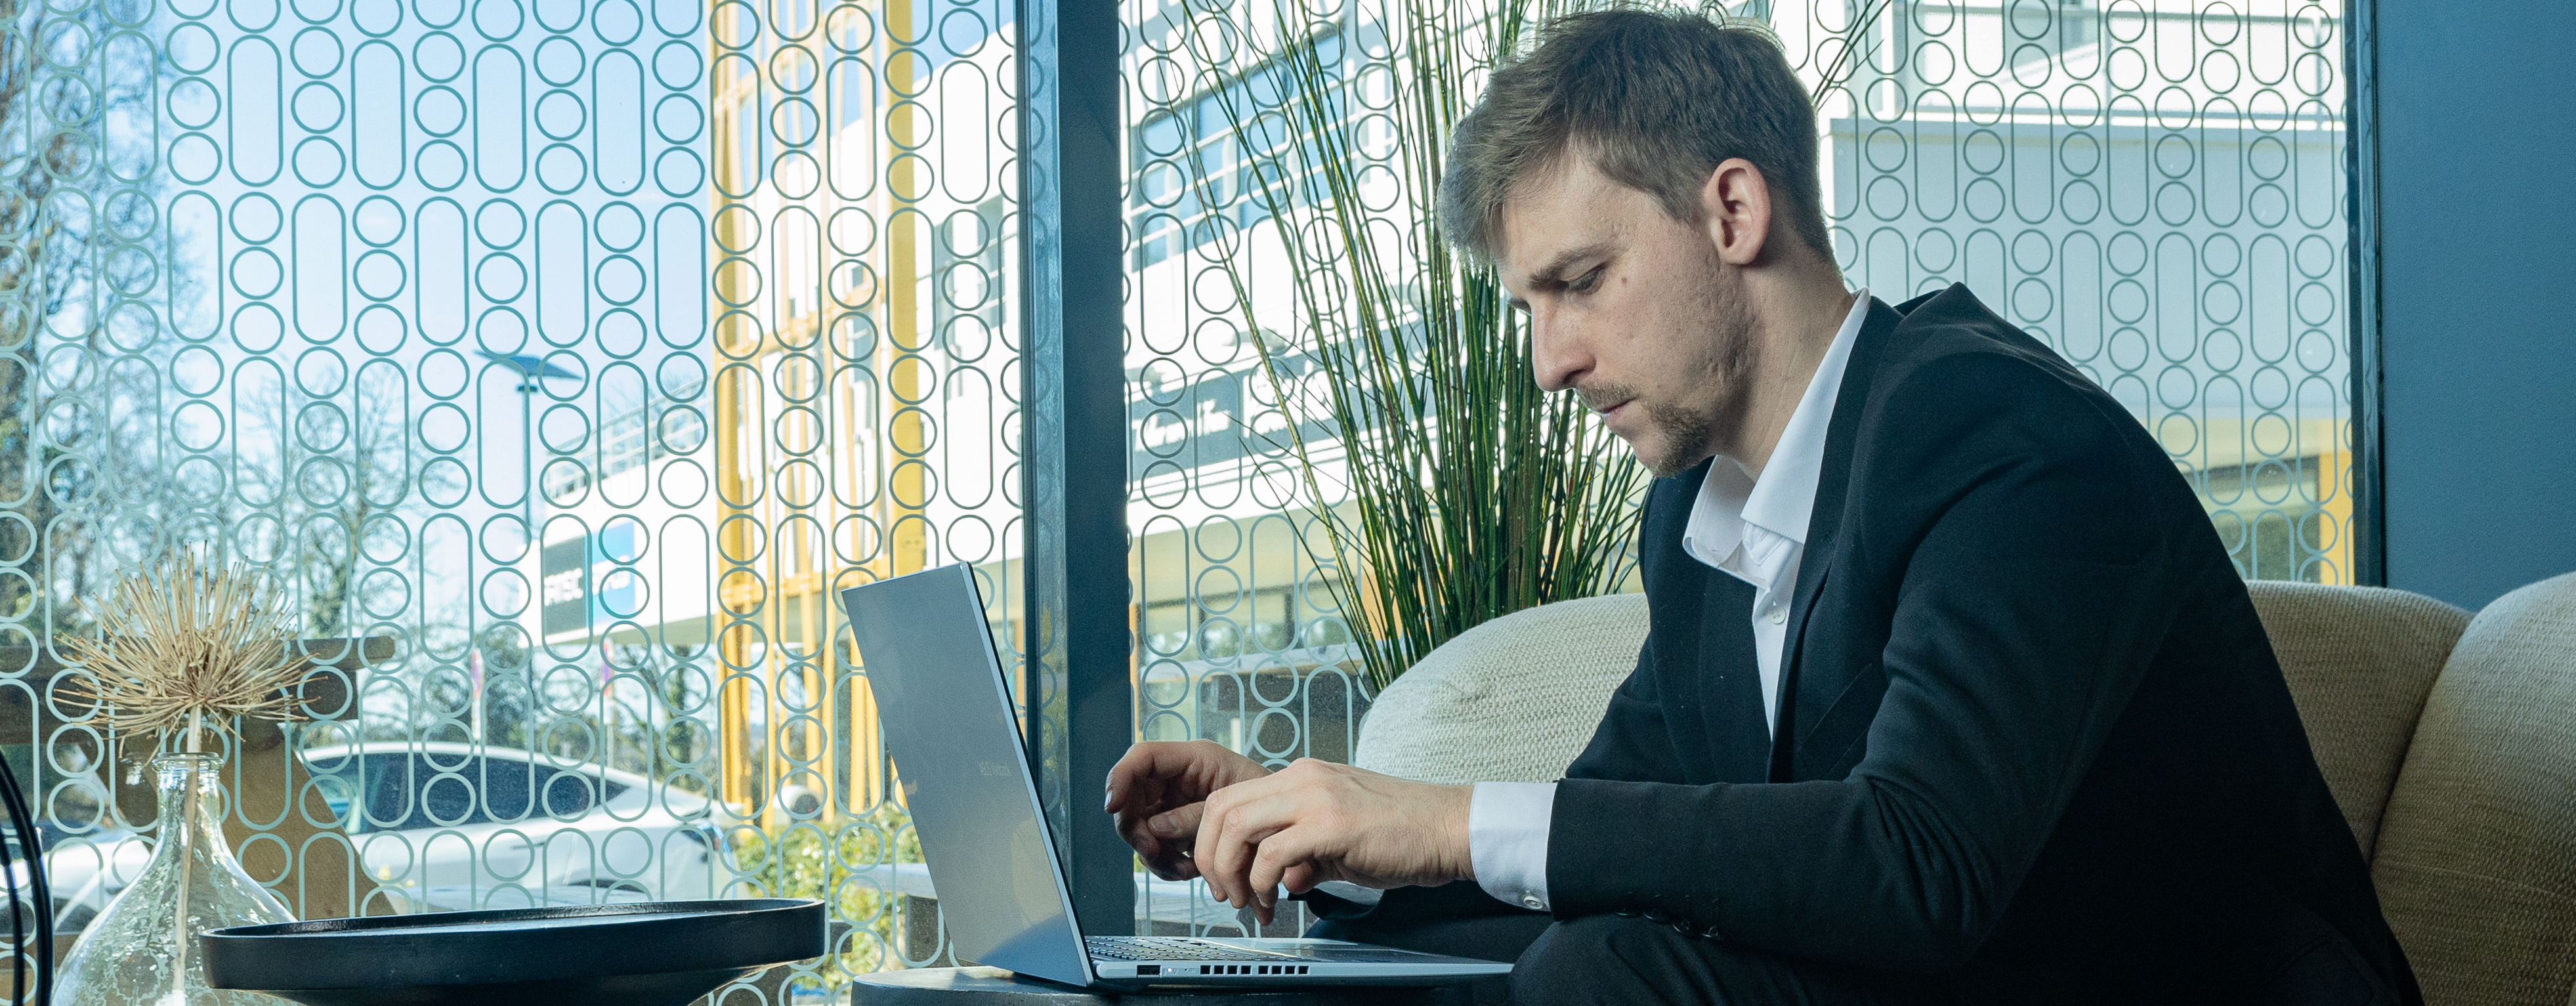
\includegraphics[width=1\linewidth]{heuzef_2025_02.jpg}
\end{figure}

\cvsection{Expériences}

\columnratio{0.5}
\begin{paracol}{2}

\cvevent{Technicien supérieur IT}{Firewall-Services}{2013 -- 2023}{Télétravail}
\begin{itemize}
\item ESN spécialisée en sécurité et en logiciels libres.
\item Maintenance d’une dizaine de parcs informatiques.
\item Maintenance en salle serveur et ZRR.
\item Assistance et formations proactives auprès des clients.
\item Supervision des infrastructures IT.
\item Rédaction de rapports et documentations technique.
\item Optimisation continue des procédures internes.
\item Analyse fonctionnelle des besoins et analyses RCA.
\item Accompagnement des équipes.
\item Résolution des situations de crise et d’urgence.

\end{itemize}

\divider

\cvevent{Freelance}{Heuzef}{2012 -- 2016}{Télétravail}
\begin{itemize}
\item Auto-entrepreneur
\item Services IT, développement web et graphisme.
\end{itemize}

\divider

\cvevent{CEMÉA Aquitaine}{Technicien IT}{2011 -- 2011}{Télétravail}
\begin{itemize}
\item Responsable SI en Service Civique.
\item Assistance et formation pédagogique et andragogique.
\end{itemize}

\switchcolumn

\cvevent{Marie de Bordeaux}{Animateur}{2011 -- 2011}{Bordeaux}
\begin{itemize}
\item Animateur pour seniors à l'atelier informatique.
\end{itemize}

\divider

\cvevent{Docteur ordinateur}{Technicien IT}{2011 -- 2011}{Bordeaux}
\begin{itemize}
\item Dépannages informatique, B2C et B2B.
\item Réparations en atelier.
\end{itemize}

\divider

\cvevent{Groupe Aquitem}{Designer Graphiste}{2011 -- 2011}{Bordeaux}
\begin{itemize}
\item Réalisation graphique, PAO et web.
\end{itemize}

\divider

\cvevent{Viacarta}{Designer Graphiste}{2011 -- 2011}{Bordeaux}
\begin{itemize}
\item Imprimeur assistant dans la chaîne graphique.
\end{itemize}

\divider

\cvevent{Divers}{}{2006 -- 2009}{Lot-et-Garonne}
\begin{itemize}
\item Divers petits jobs.
\end{itemize}

\end{paracol}

\cvsection{Centres d'intérêts}

\columnratio{0.5}
\begin{paracol}{2}

\begin{itemize}
\item Aïkidoka
\item FabLab-Manager
\item Bricoleur
\switchcolumn
\item Auto-hébergeur
\item Libriste
\item Familial
\end{itemize}

\end{paracol}

\bigskip

\raggedleft
{\textit{Dernière mise à jour \today}}\github{heuzef/cv}
\end{document}